\documentclass[10pt]{article}

% Author/preprint manuscript. Author: Alexander Revyakin.
% Before OpenReview submission, place this content into the official ICLR 2027
% style package linked from the author guidelines.
\usepackage[margin=0.78in]{geometry}
\usepackage{booktabs}
\usepackage{amsmath}
\usepackage{amssymb}
\usepackage{microtype}
\usepackage{hyperref}
\usepackage{url}
\usepackage{graphicx}
\usepackage{xcolor}
\usepackage{enumitem}
\usepackage{multirow}
\usepackage{tikz}
\usetikzlibrary{arrows.meta,positioning,fit,calc,shapes.geometric}

\title{Tiny: Verified Skill Migration for Reducing LLM Fallbacks\\in Neuro-Symbolic Question Answering}
\author{Alexander Revyakin}
\date{}

\begin{document}
\maketitle

\begin{abstract}
Large language model (LLM) cascades reduce inference cost by routing easy requests to smaller models, and distillation can further improve those models over time. We study a stricter neuro-symbolic variant: \emph{declarative facts remain external and replaceable, while only procedural skills migrate into learned parameters}. We call this process \emph{verified skill migration} (VSM). A compact local model attempts a procedural subtask, a frozen competence gate escalates uncertain cases to an LLM, and the LLM outcome becomes a training trace only after independent verification using withheld ground truth or deterministic knowledge-graph evidence. We instantiate VSM for Wikidata QA with entity linking and property mapping as migratable skills and a pinned local Wikidata snapshot as factual authority. Two skills successfully migrate, while two preregistered candidates---relation directionality and answer-type prediction---fail teacher-viability criteria and are not trained. In a fresh integrated development evaluation, the learned system saves 53 real Qwen2.5-3B calls over 351 questions and raises exact $(\mathrm{entity},\mathrm{property})$ accuracy from 34.47\% to 44.16\%. On a preregistered structural subset of the previously unopened official LC-QuAD 2.0 test split (1,074 questions), VSM reduces real teacher calls from 1,214 to 1,007, or 1.130 to 0.938 calls/question. The paired bootstrap 95\% CI for the call reduction is $[0.153,0.233]$ calls/question. Zero-call coverage rises from 25.98\% to 34.64\% while zero-call precision reaches 96.51\% (Wilson 95\% CI $[94.11,97.95]$). Exact pair accuracy has a positive point estimate, 63.59\% to 65.64\%, but its paired 95\% bootstrap CI for the difference ($[-0.28,4.47]$ percentage points) includes zero. These results support VSM as a conservative mechanism for reducing dependence on a large model without making learned weights the authoritative store of factual knowledge.
\end{abstract}

\section{Introduction}

LLM deployment increasingly relies on cascades and routers: a cheap model handles requests judged safe, while a stronger model is invoked for difficult cases. A natural extension is to train the cheap model on escalated examples so that its competence grows over time. This idea already appears in neural caching, routing, and closed-loop distillation \cite{ramirez2024cache,ong2024routellm,guo2026routenlp,yao2026mera}. The remaining architectural question is not whether a student can learn from fallbacks, but \emph{what should be allowed to migrate into the student}. This matters acutely in factual systems, where distilling answers may turn opaque model parameters into a stale or unverifiable factual store.

We investigate a different separation of responsibilities:
\begin{quote}
\centering
\textbf{Facts stay external; skills migrate inward.}
\end{quote}

We call the resulting lifecycle \emph{verified skill migration} (VSM). A small model first attempts a procedural subtask. When a preregistered competence gate rejects that attempt, a larger teacher proposes an outcome. The teacher proposal is \emph{not} trusted as a label merely because it came from a stronger model. Instead, an independent verifier checks the outcome after teacher inference. Only verified traces enter a skill buffer. A candidate skill is trained offline, retested under a frozen competence policy, and promoted only if its autonomous region expands without violating precision constraints.

The lifecycle is
\[
\begin{aligned}
\mathrm{UNKNOWN}&\rightarrow\mathrm{FALLBACK}\rightarrow\mathrm{VERIFY}
\rightarrow\mathrm{STORE\ VERIFIED\ TRACE}\\
&\rightarrow\mathrm{TRAIN\ SKILL}\rightarrow\mathrm{RETEST}
\rightarrow\mathrm{PROMOTE}.
\end{aligned}
\]
The long-run deployment objective is therefore explicit: the number of large-model calls should decrease while task quality remains stable or improves.

We instantiate the framework in ``Tiny'', a neuro-symbolic Wikidata QA system. Tiny keeps factual state in a pinned local knowledge snapshot and learns two procedural skills: entity linking and subject-conditioned property mapping. The paper makes four contributions:

\begin{enumerate}[leftmargin=*]
    \item We formulate VSM as a conservative learning pattern that combines external factual authority, post-inference verification of teacher outcomes, modular skill absorption, and frozen competence gates.
    \item We show successful migration for two distinct QA skills. Both independently reduce real Qwen fallback calls after verified learning.
    \item We report two negative preregistered skill studies. Relation directionality and answer-type prediction fail teacher-viability requirements, showing that a verifier alone does not make a skill safely migratable.
    \item We evaluate the two learned skills jointly. A preregistered formal LC-QuAD 2.0 test confirms a statistically robust reduction in teacher calls and an increase in high-precision autonomous coverage; the paired confidence interval for the accuracy difference includes zero, so we claim non-degradation rather than a significant accuracy improvement.
\end{enumerate}

Our novelty claim is deliberately narrow. Tiny is \emph{not} the first self-improving cascade. Instead, we study a specific design point in which declarative knowledge remains outside model weights while independently verified procedural fallback experience is selectively compiled into compact learned modules.

\section{Related Work}

\paragraph{LLM routing and cascades.}
RouteLLM learns routers that choose between stronger and weaker LLMs and demonstrates large cost reductions from better routing of fixed models \cite{ong2024routellm}. Routing addresses \emph{where} a request should execute but does not by itself require the cheaper model to improve.

\paragraph{Neural caching and continual distillation.}
Cache \& Distil introduces ``neural caching'': a local student is continually trained on responses from a larger LLM, while an active-learning policy decides which requests to escalate \cite{ramirez2024cache}. This is the closest established predecessor to the broad idea that future API calls can decrease because the student itself improves. RouteNLP extends this direction with a closed loop over routing, escalation failures, targeted distillation, and router retraining \cite{guo2026routenlp}. VSM differs in what is admitted to the learner: teacher output is first independently verified, and the learned modules represent procedural QA decisions rather than authoritative factual answers.

\paragraph{Verifier-backed model evolution.}
MERA is especially close in spirit. It mines failed agent invocations, obtains execution-verified teacher demonstrations, updates skills and a student adapter, and serves the student behind verifier-backed fallback \cite{yao2026mera}. OVCSD likewise retains only outcome-verified successful teacher continuations for agent self-distillation \cite{xia2026ovcsd}. Tiny should therefore not be framed as the first verifier-backed or outcome-verified self-improving system. Our narrower focus is a neuro-symbolic decomposition where factual state remains external, individual procedural skills are trained as separate learned components, and deployment is evaluated by displacement of actual LLM calls under fixed competence gates.

\paragraph{Declarative versus procedural memory.}
Anything2Skill separates external declarative evidence from reusable procedural skills, compiling heterogeneous sources into an explicit SkillBank \cite{pan2026anything2skill}. Tiny explores a complementary location in the design space: procedural skills migrate into compact model weights, whereas the declarative factual source remains external and queryable.

\paragraph{Knowledge-graph question answering.}
Wikidata provides the external factual substrate \cite{vrandecic2014wikidata}. We use Mintaka \cite{sen2022mintaka}, SimpleQuestions-derived supervision \cite{bordes2015simplequestions} in the property experiments, and LC-QuAD 2.0 \cite{dubey2019lcquad2}. Our formal claim is \emph{not} full LC-QuAD 2.0 QA performance. It is explicitly restricted to a preregistered single-direct-$(QID,PID)$ structural subset compatible with the pinned Wikidata snapshot.



\begin{table}[t]
\centering
\caption{Positioning relative to the closest systems. A checkmark denotes an
explicit design property in the cited work; ``--'' means that the property is
not an explicit design objective, not that the system is incompatible with it.
The table is a positioning aid, not a priority claim.}
\label{tab:related-comparison}
\scriptsize
\setlength{\tabcolsep}{3.0pt}
\resizebox{\linewidth}{!}{%
\begin{tabular}{lccccc}
\toprule
System &
Student weights improve &
Outcome-verified supervision &
External factual authority &
Explicit procedural memory &
Future strong-model use measured \\
\midrule
RouteLLM \cite{ong2024routellm} &
-- & -- & -- & -- & \checkmark \\
Cache \& Distil \cite{ramirez2024cache} &
\checkmark & -- & -- & -- & \checkmark \\
RouteNLP \cite{guo2026routenlp} &
\checkmark & -- & -- & -- & \checkmark \\
MERA \cite{yao2026mera} &
\checkmark & \checkmark & -- & \checkmark & \checkmark \\
OVCSD \cite{xia2026ovcsd} &
\checkmark & \checkmark & -- & -- & -- \\
Anything2Skill \cite{pan2026anything2skill} &
--$^\dagger$ & -- & \checkmark & \checkmark & -- \\
\textbf{Tiny / VSM} &
\textbf{\checkmark} & \textbf{\checkmark} & \textbf{\checkmark} &
\textbf{\checkmark} & \textbf{\checkmark} \\
\bottomrule
\end{tabular}%
}

\vspace{1mm}
\begin{minipage}{0.97\linewidth}
\scriptsize
$^\dagger$Anything2Skill compiles reusable procedures into an external SkillBank
rather than improving a compact student from fallback experience. OVCSD retains
only outcome-verified successful continuations for agent self-distillation,
making verification-before-update explicit prior art. Tiny's claim is therefore
about the combined neuro-symbolic design point, not any individual column.
\end{minipage}
\end{table}

\paragraph{Positioning of the contribution.}
Table~\ref{tab:related-comparison} makes the intended claim boundary explicit.
None of the ingredients is new in isolation. Routing and fallback displacement
are established; neural caching and RouteNLP improve cheaper models from
escalations; MERA and OVCSD establish outcome-verified adaptation; and
Anything2Skill explicitly separates declarative evidence from reusable
procedures. Tiny tests their conservative combination in a neuro-symbolic
setting: factual authority is kept external, a teacher-produced procedural target
must pass an outcome check before entering a learning buffer, separate compact
modules absorb repeated procedural decisions, and frozen stage-specific gates
determine whether those modules may replace the LLM. We therefore make no
``first self-improving cascade'', ``first verified distillation'', or
``first procedural-memory'' claim.



\section{Verified Skill Migration}

\begin{figure}[t]
\centering
\resizebox{\linewidth}{!}{%
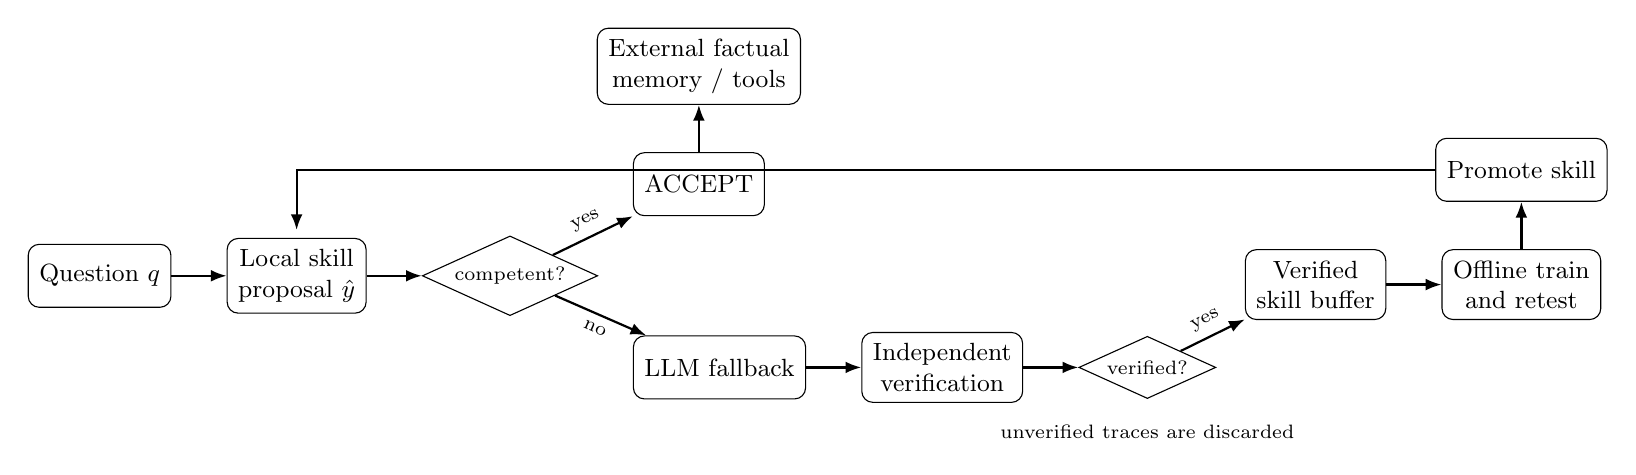
\begin{tikzpicture}[
  node distance=6mm and 7mm,
  box/.style={draw, rounded corners, align=center, minimum height=8mm, inner sep=4pt, font=\small},
  gate/.style={draw, diamond, aspect=2.2, align=center, inner sep=1.5pt, font=\scriptsize},
  arr/.style={-{Latex[length=2mm]}, thick},
  note/.style={font=\scriptsize, align=center}
]
\node[box] (q) {Question $q$};
\node[box, right=of q] (skill) {Local skill\\proposal $\hat y$};
\node[gate, right=of skill] (gate) {competent?};
\node[box, above right=5mm and 10mm of gate] (accept) {ACCEPT};
\node[box, below right=5mm and 10mm of gate] (teacher) {LLM fallback};
\node[box, right=of teacher] (verify) {Independent\\verification};
\node[gate, right=of verify] (ok) {verified?};
\node[box, above right=4mm and 8mm of ok] (buffer) {Verified\\skill buffer};
\node[box, right=of buffer] (train) {Offline train\\and retest};
\node[box, above=of train] (promote) {Promote skill};
\node[box, above=of accept] (memory) {External factual\\memory / tools};

\draw[arr] (q) -- (skill);
\draw[arr] (skill) -- (gate);
\draw[arr] (gate) -- node[above,sloped,note]{yes} (accept);
\draw[arr] (gate) -- node[below,sloped,note]{no} (teacher);
\draw[arr] (teacher) -- (verify);
\draw[arr] (verify) -- (ok);
\draw[arr] (ok) -- node[above,sloped,note]{yes} (buffer);
\draw[arr] (buffer) -- (train);
\draw[arr] (train) -- (promote);
\draw[arr] (promote.west) -| ($(skill.north)+(0,0.1)$);
\draw[arr] (accept) -- (memory);
\node[note, below=2mm of ok] {unverified traces are discarded};
\end{tikzpicture}%
}
\caption{Verified skill migration. The LLM is a proposer, not an authority. Only independently verified fallback outcomes enter the learning buffer. Factual state remains external.}
\label{fig:vsm}
\end{figure}

\subsection{System decomposition}
For a question $q$, Tiny decomposes a simple factual QA decision into procedural stages. The two promoted learned stages are entity linking, which selects a Wikidata subject $e$, and property mapping, which selects a property $p$ conditioned on $e$. Deterministic graph access then retrieves factual values from external memory using $(e,p)$. Learned models are therefore never treated as the authoritative factual store.

At stage $s$, Tiny computes a local proposal $\hat y_s$ and a frozen competence decision
\[
g_s(q,\hat y_s,\phi_s)\in\{\mathrm{ACCEPT},\mathrm{FALLBACK}\},
\]
where $\phi_s$ contains deterministic evidence available to the stage. If the gate returns FALLBACK, the LLM proposes an outcome. Importantly, the model used for fallback may be far larger than the local skill model, but its output still has no privileged epistemic status.


\subsection{Independent verification and admission}
Here ``independent'' has a narrow operational meaning: the admission decision
does not use the teacher's confidence, hidden state, or a second prompt asking
the same teacher to judge itself. The proposed target is checked only
\emph{after} teacher inference against an external outcome signal. Depending on
the experiment, that signal is either withheld benchmark ground truth revealed
after inference or deterministic evidence from the pinned knowledge graph. This
is an offline experimental instantiation of outcome verification; it should not
be read as a claim that benchmark gold is available in a production system.

Let $y_T$ be the fallback proposal and let $z$ denote evidence unavailable to the teacher during its inference pass. Depending on the experiment, $z$ is a withheld benchmark label or deterministic evidence from the pinned KG. The verifier returns
\[
v(q,y_T,z)\in\{0,1\}.
\]
Only traces with $v=1$ are admitted:
\[
\mathcal D_{\mathrm{verified}}=\{(q,y_T):v(q,y_T,z)=1\}.
\]
This timing constraint matters: gold labels used for verification are opened only \emph{after} teacher inference. The verifier is thus independent of the teacher's proposal process even when benchmark supervision provides the reference label.

\subsection{Skill promotion}
Learning is offline in the present study. A candidate skill is trained only on its verified buffer and is evaluated under a preregistered competence policy. We do not select checkpoints or retune acceptance thresholds on the protected holdout. A skill is promoted only if coverage/fallback metrics improve while precision constraints remain satisfied. Failed skill candidates are closed rather than repeatedly rescued on the same protected sample.

\section{Experimental Setup}

\subsection{Pinned factual memory and models}
All experiments use a Wikidata snapshot dated 2026-08-17, SHA1
\texttt{9888bb6c50f1310b229c077084991f3ea6e6406a}, transformed into a local TinyMemory plus deterministic accelerators. The snapshot is held fixed across all promoted skills and integrated evaluations.

The fallback teacher is Qwen2.5-3B-Instruct at revision
\texttt{\small aa8e72537993ba99e69dfaafa59ed015\allowbreak b17504d1}
(3,085,938,688 parameters) \cite{qwen2024qwen25}. The directionality stress test additionally evaluates Qwen2.5-7B-Instruct. The promoted entity model has 109,482,240 parameters. The promoted property model has 29,193,768 parameters. Both learned modules can reside simultaneously in one process (138,676,008 total learned parameters) before fallback is invoked.

\subsection{Frozen competence policies}
\paragraph{Entity.}
The deployed entity skill accepts only when (i) the direct local top-1 and final evidence-aware top-1 entity agree, (ii) the best relation-evidence rank is at most five, and (iii) the selected entity has at least 20 properties in TinyMemory. Otherwise the stage falls back to Qwen.

\paragraph{Property.}
Properties are ranked over the actual property set of the resolved subject. The deployed property skill accepts iff lexical subject-conditioned top-1 agrees with neural subject-conditioned top-1. No learned confidence threshold is tuned on the protected evaluation split.

\subsection{Training recipes}
The entity skill is trained from 788 verified traces (314 corrections and 474 reinforcements) for three epochs with learning rate $10^{-5}$, weight decay $0.01$, contrastive temperature $0.05$, batch size four rows, and seed 1534. There is no early stopping or checkpoint selection.

The property skill is trained from 651 verified traces (302 corrections and 349 reinforcements) for three epochs with learning rate $10^{-5}$, weight decay $0.01$, temperature $0.05$, batch size eight rows, and seed 1542. Again, there is no early stopping or checkpoint selection.


\subsection{Preregistered evaluation questions}
The integrated study is organized around three deployment questions rather than
a generic ``does accuracy improve?'' hypothesis:
\begin{description}[leftmargin=1.4cm,style=nextline]
    \item[RQ1.] Do the learned skills reduce the number of \emph{actual} teacher
    invocations on paired questions?
    \item[RQ2.] Does exact $(e,p)$ hybrid accuracy remain within the frozen
    accuracy-retention gate (no more than a 1 percentage-point point-estimate drop)?
    \item[RQ3.] Does the learned zero-call region remain precise enough to be
    trusted (PRIMARY: precision $\geq85\%$ with at least 20 autonomous rows;
    STRONG: precision $\geq90\%$ with at least 40)?
\end{description}
The formal test reuses these frozen criteria without threshold, prompt, or
checkpoint changes after the fresh development run.

\subsection{Evaluation metrics}
Our primary systems metric is the number of \emph{real} Qwen calls, not a simulated routing proxy. Because a question may invoke fallback at both entity and property stages, calls/question can exceed one. We also report exact subject-property pair accuracy, stage accuracies, any-LLM-call rate, and autonomous zero-call coverage. Zero-call precision is the exact pair precision among questions answered without any teacher invocation.

\subsection{Scientific protocol}
The experimental protocol is designed to make post-hoc adaptation difficult:
\begin{itemize}[leftmargin=*]
    \item preregistration artifacts are written before protected labels or teacher outcomes are inspected;
    \item teacher traces are persisted before gold labels are opened for verification;
    \item only independently verified traces enter learning buffers;
    \item no threshold tuning, early stopping, or checkpoint selection is performed on protected holdouts;
    \item each run stores logs, result JSON, traces/predictions, executed script snapshots, and SHA256 manifests;
    \item the official LC-QuAD 2.0 test split is first accessed only after the formal-test preregistration is written;
    \item after the formal test, no benchmark tuning or rescue run is performed.
\end{itemize}

\section{Skill Migration Studies}

\begin{table}[t]
\centering
\caption{Skill-level studies before integrated evaluation. ``Calls'' are real Qwen calls under the corresponding frozen hybrid policy.}
\label{tab:skills}
\small
\begin{tabular}{lllll}
\toprule
Skill & Outcome & Verified signal & Before & After \\
\midrule
Entity linking & PASS & 788 traces & 148/200 calls & 140/200 calls \\
Property mapping & PASS & 651 traces & 473/800 calls & 322/800 calls \\
Directionality & FAIL & 79.69\% overall & \multicolumn{2}{l}{inverse verified coverage 43.60\%} \\
Answer type & FAIL & 67.79\% precision & \multicolumn{2}{l}{minority classes collapse toward ENTITY} \\
\bottomrule
\end{tabular}
\end{table}

\subsection{Entity linking}
The first promoted skill is trained from independently verified Mintaka TRAIN-derived traces. On a 200-question internal development set, actual Qwen calls fall from 148 to 140 (74\% to 70\%) while hybrid accuracy rises from 55.5\% to 58.0\%. Autonomous ACCEPT coverage increases from 26\% to 30\% while precision remains above 90\%.

\subsection{Property mapping}
Property candidates are conditioned on the resolved subject and combine lexical and neural ranking. On an 800-question disjoint holdout, learning raises ACCEPT coverage from 40.75\% to 59.63\%, ACCEPT precision from 91.10\% to 95.60\%, and resolver accuracy from 63.5\% to 79.63\%. A subsequent real-teacher run on the frozen holdout reduces Qwen calls from 473 to 322 while hybrid accuracy rises from 81.38\% to 87.63\%.

\subsection{Negative skill studies}
\paragraph{Relation directionality.}
After weaker teacher variants fail, a fresh preregistered Qwen2.5-7B run on 1,600 examples reaches 79.69\% overall verified accuracy. Direct relations reach 90.43\% verified coverage, but inverse relations reach only 43.60\%. The preregistered gate fails and the branch is closed without training.

\paragraph{Answer-type prediction.}
On 1,600 fresh Mintaka TRAIN questions, Qwen2.5-3B reaches 67.79\% teacher precision. ENTITY coverage is 99.48\%, but BOOLEAN, DATE, and NUMBER coverage is only 31.02\%, 13.59\%, and 10.68\%, respectively. The teacher strongly overpredicts ENTITY, so the candidate skill is not trained.

These negative results constrain the interpretation of VSM. Independent verification is necessary but not sufficient. The teacher must generate a sufficiently accurate and sufficiently broad verified supervision distribution for a skill to be worth absorbing.

\section{Integrated Evaluation}

\subsection{Fresh development evaluation}
After both successful skills are frozen, we load them simultaneously and evaluate the complete chain. We construct a fresh Mintaka TRAIN-derived structural subset after excluding every previously exposed Mintaka pool and normalized duplicate. The original preregistration targeted 400 rows, but only 351 satisfy all frozen freshness and unique-direct-edge constraints; the first run stops before any model/teacher outcome is produced. The engineering-fixed run uses \emph{all} 351 qualifying rows, without outcome-based selection.

\begin{table}[t]
\centering
\caption{Integrated fresh development evaluation (351 questions).}
\label{tab:dev}
\begin{tabular}{lrr}
\toprule
Metric & Baseline & Learned \\
\midrule
Real Qwen calls & 568 & \textbf{515} \\
Calls / question & 1.618 & \textbf{1.467} \\
Entity hybrid accuracy & 61.25\% & \textbf{66.67\%} \\
Property PID accuracy & 39.32\% & \textbf{50.43\%} \\
Exact $(e,p)$ accuracy & 34.47\% & \textbf{44.16\%} \\
Zero-call coverage & 6.84\% & \textbf{9.69\%} \\
Zero-call precision & 66.67\% & \textbf{85.29\%} \\
\bottomrule
\end{tabular}
\end{table}

The learned pipeline saves 53 real teacher calls and improves the point estimate of exact pair accuracy by 9.69 percentage points. The preregistered PRIMARY development gate passes; the more demanding STRONG gate fails because zero-call sample size and precision do not reach its higher thresholds.

\subsection{Preregistered formal LC-QuAD 2.0 test}
The official LC-QuAD 2.0 test split is first accessed after the final preregistration is frozen. The formal scope is defined by query structure and snapshot compatibility, not by any model output. Eligible rows have (i) a nonempty natural-language question, (ii) exactly one distinct \texttt{wd:Q...} constant, (iii) exactly one distinct direct \texttt{wdt:P...} property, (iv) exactly one explicit direct triple of the form \texttt{wd:Q... wdt:P... ?variable}, and (v) a property present in the frozen catalog and in the pinned snapshot's property set for that subject. All 1,074 qualifying rows are used. We emphasize that this is a subset-conditioned formal claim, not full-benchmark LC-QuAD 2.0 QA performance.

\begin{table}[t]
\centering
\caption{Formal LC-QuAD 2.0 test results on the preregistered 1,074-row structural subset.}
\label{tab:test}
\begin{tabular}{lrr}
\toprule
Metric & Baseline & Learned \\
\midrule
Real Qwen calls & 1,214 & \textbf{1,007} \\
Calls / question & 1.130 & \textbf{0.938} \\
Any-LLM-call rate & 73.93\% & \textbf{65.27\%} \\
Entity hybrid accuracy & 72.53\% & \textbf{74.02\%} \\
Property PID accuracy & 66.57\% & \textbf{68.99\%} \\
Exact $(e,p)$ accuracy & 63.59\% & \textbf{65.64\%} \\
Zero-call coverage & 25.98\% & \textbf{34.64\%} \\
Zero-call precision & 93.91\% & \textbf{96.51\%} \\
\bottomrule
\end{tabular}
\end{table}

The learned pipeline saves 207 actual Qwen calls. Calls/question falls by 0.193, a 17.1\% relative reduction against the baseline call intensity. Of the 207 saved calls, 101 come from the entity stage (689$\rightarrow$588) and 106 from the property stage (525$\rightarrow$419). Autonomous zero-call answers increase from 279 to 372 under the policy-level definition. Both preregistered PRIMARY and STRONG formal-test gates pass.

\begin{table}[t]
\centering
\caption{Paired mechanism audit on the same 1,074 formal test questions. This is
descriptive decomposition, not a factorial ablation: both learned skills change
simultaneously between the two system versions.}
\label{tab:paired-audit}
\small
\begin{tabular}{lrrr}
\toprule
Paired quantity & Baseline & Learned & Net / transition \\
\midrule
Entity-stage teacher calls & 689 & 588 & $-101$ \\
Property-stage teacher calls & 525 & 419 & $-106$ \\
Entity gate ACCEPT rate & 35.75\% & 45.16\% & $+9.40$ pp \\
Property gate ACCEPT rate & 50.93\% & 60.80\% & $+9.87$ pp \\
\midrule
Questions using fewer total calls & -- & -- & 301 (28.0\%) \\
Questions using the same calls & -- & -- & 654 (60.9\%) \\
Questions using more total calls & -- & -- & 119 (11.1\%) \\
\midrule
Fallback $\rightarrow$ zero-call & -- & -- & 136 \\
Zero-call $\rightarrow$ fallback & -- & -- & 43 \\
Wrong $\rightarrow$ correct pair & -- & -- & 96 \\
Correct $\rightarrow$ wrong pair & -- & -- & 74 \\
\bottomrule
\end{tabular}
\end{table}

The paired audit shows that fallback displacement is not attributable to a
single stage: entity and property contribute 101 and 106 saved calls,
respectively. The learned version uses fewer calls on 301 questions and more on
119, yielding the net reduction. Likewise, zero-call status is gained on 136
questions and lost on 43, while exact-pair correctness flips in both directions
(96 improvements versus 74 regressions). This last asymmetry explains the
positive accuracy point estimate while also motivating the paired uncertainty
analysis below.


\subsection{Paired statistical analysis}
Because baseline and learned systems are evaluated on identical questions, we use paired resampling over question IDs. A 100,000-sample paired bootstrap gives a 95\% CI of $[0.153,0.233]$ calls/question for the reduction in total teacher calls. The zero-call coverage increase is 8.66 percentage points with paired-bootstrap 95\% CI $[6.24,11.08]$ points. Learned zero-call precision is 359/372 = 96.51\%, with Wilson 95\% CI $[94.11,97.95]$.

The exact pair-accuracy point estimate increases by 2.05 percentage points, but the paired bootstrap 95\% CI is $[-0.28,4.47]$ points. The discordant-pair counts are 96 questions corrected by the learned system versus 74 questions made incorrect; an exact McNemar test gives $p=0.107$. We therefore do \emph{not} claim a statistically significant accuracy improvement. The supported formal claim is that VSM substantially reduces real fallback use and expands high-precision autonomy while satisfying the preregistered point-estimate accuracy-retention gate. The lower bootstrap bound of $-0.28$ percentage points also remains above the frozen $-1$ point retention margin, although this paired interval was added as a post-hoc uncertainty analysis rather than as the preregistered decision rule.

Candidate recall on the formal structural subset is 90.88\%, placing an upper bound on downstream entity resolution independent of the competence policy.

\section{Discussion}

\subsection{What is supported}
Across two procedural skills, verified fallback experience can be absorbed into compact local models in a way that measurably displaces future teacher calls. The effect survives joint deployment: on the formal test, the learned system uses the teacher on fewer questions, uses fewer total calls when it does fall back, and answers a larger fraction autonomously at high precision.

The result is stronger than a pure router comparison because the cheap model's competence changes after verified experience. It is narrower than general self-improving-agent claims because only two procedural skills migrate and factual truth remains delegated to external memory.

\subsection{A boundary condition: verifiability is not enough}
The directionality and answer-type experiments show that VSM cannot simply attach a verifier to any skill and expect improvement. A practical approximation is
\[
\mathrm{migration\ viability}\approx
\mathrm{verifiability}\times
\mathrm{teacher\ signal\ quality}\times
\mathrm{learnability}\times
\mathrm{safe\ gating}.
\]
If any factor is weak, the appropriate action may be to keep the skill in FALLBACK rather than force a distillation run.

\subsection{Why keep facts external?}
The architecture makes factual updates independent of weight updates, preserves explicit provenance, and permits a failed learned skill to be disabled without modifying the factual store. This does not guarantee factual correctness---the external store and deterministic tooling can themselves be wrong---but it makes the authority boundary inspectable and replaceable.

\subsection{Relation to MERA and neural caching}
Cache \& Distil establishes that a student can learn from LLM escalations and thereby reduce future API use \cite{ramirez2024cache}. MERA goes further with execution-verified demonstrations and verifier-backed deployment \cite{yao2026mera}. Tiny's contribution should be understood as a specific neuro-symbolic specialization: independent verification gates trace admission, procedural competencies migrate as modular skills, declarative facts remain outside the learned models, and factual retrieval is deterministic after procedural resolution. The formal test quantifies the resulting displacement of real fallback calls.

\section{Limitations}
The formal test covers only the preregistered LC-QuAD 2.0 subset with one direct subject-property relation compatible with the pinned snapshot. It should not be interpreted as full LC-QuAD 2.0 QA performance. The use of gold SPARQL to define structural scope is intentional and preregistered, but it means the formal claim is conditional on that scope. Exact entity-candidate recall on this subset is 90.88\%, which places a hard ceiling on downstream entity resolution before any competence policy or teacher decision is considered.

Only two skills successfully migrate, both within KG query resolution. Generalization to long-horizon reasoning, free-form generation, tool orchestration, or domains without reliable verification remains open. The main fallback teacher is a single model family; teacher choice may affect viability. The directionality stress test suggests that merely increasing teacher size is not always enough.

The present system trains offline rather than updating weights continually in production. We also report calls and teacher-generation time from a single hardware/software stack rather than a provider-normalized monetary cost. Production deployment would require distribution-shift monitoring, verifier audits, replay-based regression tests, rollback, and protection against corruption of the external factual store.

Finally, the paired formal-test analysis provides strong evidence for fallback reduction and autonomous-coverage growth, but not for a statistically significant accuracy increase. Our conclusion is therefore cost/LLM-dependence reduction while retaining accuracy, not accuracy superiority.

\section{Ethics Statement}
This work uses public research benchmarks and a public Wikidata snapshot and collects no new human-subject data. The main risks are methodological rather than application-specific: overclaiming benchmark scope, treating a verifier as infallible, or deploying a stale or corrupted external knowledge snapshot. We mitigate these risks by stating the structural test scope explicitly, recording negative experiments and invalidated development artifacts, pinning provenance by checksum, and keeping factual authority replaceable rather than embedding it as an uninspectable source of truth in learned weights.

\section{Reproducibility Statement}
Every reported experimental run stores a preregistration, full run log, result JSON, prediction or trace files where applicable, a snapshot of the executed Python script, and a SHA256 artifact manifest. Model revisions, parameter counts, Wikidata snapshot hashes, seeds, and competence policies are pinned in the artifacts. Appendix~\ref{app:provenance} lists key formal-test hashes and Appendix~\ref{app:protocol} summarizes the protected-data protocol. An anonymized reproduction bundle will include executable scripts and instructions for rebuilding TinyMemory from public sources.

\section{AI Use Statement}
Generative AI tools were used to propose and refine hypotheses, provide feedback on experimental methodology, implement and debug experimental scripts, assist with literature discovery and comparison, interpret and audit experimental outputs, perform statistical-analysis coding, and draft/edit manuscript text. These uses include activities for which ICLR 2027 requires disclosure. Experimental runs were executed in the author's local environment. AI-generated code and conclusions were checked against stored preregistrations, raw traces, logs, checksums, and independently computed metrics. Protected benchmark outcomes were not used for post-hoc threshold selection, checkpoint selection, or rescue tuning after the corresponding preregistration. The author reviewed the AI-assisted work and takes responsibility for the final methodology, claims, code, statistics, and manuscript.

\section{Conclusion}
Verified skill migration is a conservative neuro-symbolic learning pattern in which factual authority remains external while procedural abilities are learned from independently verified fallback experience. Entity linking and property mapping successfully migrate into compact local models; two other candidate skills fail before training, revealing a boundary of the method. On a preregistered 1,074-question structural subset of the previously unopened LC-QuAD 2.0 test split, the learned system saves 207 real Qwen calls, reduces calls/question by 17.1\%, and increases autonomous coverage by 8.66 percentage points at 96.51\% precision. The accuracy difference is consistent with the preregistered accuracy-retention criterion but is not statistically significant. The robust empirical result is fallback displacement rather than accuracy superiority: the learned system invokes the teacher substantially less often while expanding a high-precision autonomous region, and the paired analysis is consistent with the frozen accuracy-retention requirement. This supports a path toward systems whose dependence on general-purpose LLMs declines with verified experience while factual state remains explicit, inspectable, and replaceable.

\bibliographystyle{plain}
\bibliography{references}

\appendix

\section{Experimental Lineage and Guardrails}\label{app:protocol}
The reported sequence contains successful and unsuccessful branches rather than only cherry-picked positive studies. The promoted entity skill is followed by a clean property-training/holdout lineage and then by a real-teacher property call-rate study. Directionality is tested with multiple preregistered teacher settings and closed after Qwen2.5-7B still fails the inverse-relation criterion. Answer-type prediction is likewise closed after the first scientifically valid teacher-viability study fails. Neither failed branch is trained on its protected sample.

The integrated DEV run excludes all previously exposed Mintaka pools and normalized duplicates. Its first engineering attempt stops before baseline, learned, or teacher inference because only 351 rows satisfy the frozen eligibility rule instead of the expected 400. The corrected run uses all 351 rows and does not change models, prompts, gates, or outcome thresholds.

The formal LC-QuAD 2.0 test is first downloaded after \texttt{PREREG\_TEST.json} is written. The formal result is frozen after that single scientific run; no threshold, prompt, checkpoint, or row-selection tuning is performed afterward.


\section{Audit of a Superseded Development Artifact}\label{app:superseded}
During development of the property pipeline, we detected that an early stored
subject-conditioned ranking artifact from v1.50.2 exposed ranking availability
only when the target property was present in the candidate set. This made a
subsequent early analysis scientifically invalid because ranking availability
was indirectly conditioned on gold presence. We excluded that result from all
claims in this paper and rebuilt the clean property pipeline directly from
TinyMemory subject property sets, with ranking performed before gold access.
The reported clean lineage begins with the corrected holdout gate and learned
property runs; the contaminated aggregate result is neither used for model
selection nor cited as evidence. We include this note because the invalid
artifact may remain visible in a complete experimental archive.

\section{Formal Test Provenance}\label{app:provenance}
The formal run uses the official LC-QuAD 2.0 test split source and records all
protected artifacts by checksum. For legibility, hashes are line-broken below;
the underlying values are contiguous hexadecimal strings.

\begin{description}[leftmargin=2.7cm,style=nextline,font=\normalfont\bfseries]
\item[test source SHA256]
\texttt{ba1500efe6308ba8\allowbreak 6af7f91033e18477\allowbreak 8204dca7ba358c77\allowbreak 222626ae6bd3454d}
\item[Sealed gold SHA256]
\texttt{74d8d7d457d311ed\allowbreak 59efcaca688d1d96\allowbreak 53c6857f91a2d0dd\allowbreak 0d5c29fa91cf0e16}
\item[Formal script SHA256]
\texttt{084c3cc51d5cdc9a\allowbreak f03e2d27d0371131\allowbreak 29955c5882b9b0d3\allowbreak 13773693fa82d0eb}
\item[Learned entity SHA256]
\texttt{82cdae409e28b7c3\allowbreak 92fea7d37872dc6d\allowbreak 82f4a306c5e6dc46\allowbreak 46b060837f6d8e4b}
\item[Learned property SHA256]
\texttt{fec50285e9727d9e\allowbreak e7fa1b4b1f60b170\allowbreak 2bea1f61c14298f3\allowbreak f61d79d1e8eb4083}
\end{description}

\section{Formal Test Paired Statistics}
For exact pair accuracy, baseline correct/learned wrong occurs on 74 questions, while baseline wrong/learned correct occurs on 96. The exact McNemar $p$-value is 0.107. With 100,000 paired bootstrap replicates (seed 1562), the accuracy-difference 95\% interval is $[-0.28,4.47]$ percentage points, the calls/question-reduction interval is $[0.153,0.233]$, and the zero-call-coverage-difference interval is $[6.24,11.08]$ percentage points.

The baseline zero-call precision is 262/279 = 93.91\% (Wilson 95\% CI $[90.46,96.16]$), and the learned zero-call precision is 359/372 = 96.51\% (Wilson 95\% CI $[94.11,97.95]$).

\section{Key Artifact Summary}
\begin{table}[h]
\centering
\small
\begin{tabular}{lll}
\toprule
Artifact / result & Value & Role \\
\midrule
Wikidata snapshot & 2026-08-17 & external factual authority \\
Entity learned model & 109,482,240 params & promoted skill \\
Property learned model & 29,193,768 params & promoted skill \\
Fallback teacher & Qwen2.5-3B-Instruct & proposer on FALLBACK \\
Formal test rows & 1,074 & all qualifying structural rows \\
Formal calls saved & 207 & primary deployment effect \\
Formal zero-call precision & 96.51\% & competence-gate safety signal \\
\bottomrule
\end{tabular}
\end{table}

\end{document}
